\chapter{Progettazione e codifica}
\label{cap:progettazione-codifica}

\intro{In questo capitolo saranno  descritte le attività di progettazione e codifica dell'applicativo.
Inoltre verranno descritte le tecnologie utilizzate durante lo sviluppo del progetto, le scelte architettuturali e i componenti sviluppati.
}\\

\section{Tecnologie utilizzate}
\label{sec:tecnologie-strumenti}

Di seguito viene data una panoramica delle tecnologie utilizzate durante lo sviluppo del progetto di stage.

\subsection{Frontend}\label{subsec:frontend}
\subsubsection{Vue.js}\label{subsubsec:vue}
Vue.js è un framework JavaScript progressivo e reattivo, utilizzato per lo sviluppo di interfacce utente dinamiche e moderne. 
Creato da Evan You, Vue.js è apprezzato per la sua semplicità d'uso e flessibilità. Con un sistema di reattività basato su un modello di oggetti e dipendenze, 
Vue.js rende facile il monitoraggio e l'aggiornamento automatico dell'interfaccia utente in base ai cambiamenti di stato dei dati. La sua architettura basata 
su componenti consente di organizzare il codice in moduli riutilizzabili e autonomi, semplificando la creazione di applicazioni complesse. 
Grazie alle direttive, è possibile arricchire il DOM con funzionalità reattive, mentre il sistema di routing agevola la creazione di single page application. 
Con una crescita costante della comunità di sviluppatori, Vue.js è diventato un'opzione popolare nel mondo dello sviluppo frontend.
Per il mio progetto sono andato ad utilizzare la versione 3 di Vue.js, insieme allo script setup, che è una nuova sintassi per definire componenti progettata per semplificare la struttura del codice e migliorare la leggibilità.

\subsubsection{Typescript}\label{subsubsec:typescript}
TypeScript è un linguaggio di programmazione open-source sviluppato da Microsoft. Si basa su JavaScript e offre tipizzazione statica opzionale, 
consentendo agli sviluppatori di specificare tipi per variabili, parametri di funzioni e oggetti. Questa caratteristica aiuta a individuare errori e a migliorare 
la manutenibilità del codice. TypeScript viene poi compilato in JavaScript, rendendolo compatibile con tutti i browser e le piattaforme. 
Con una sintassi familiare per i programmatori JavaScript, TypeScript è adottato sempre di più nella community sia per lo sviluppo frontend che backend.
All'interno del mio progetto sono andato a creare per la parte frontend una cartella chiamata types che contiene un file typescript contenente tutti i tipi utilizzati all'interno del progetto.
\subsubsection{Vite.js}\label{subsubsec:vite}
Vite.js è un build tool utilizzato per lo sviluppo di applicazioni web. È stato creato da Evan You, lo stesso creatore di Vue.js, e si basa su rollup.js.
Vite.js è stato progettato per essere veloce, semplice da utilizzare e facile da configurare. La sua velocità è dovuta al fatto che utilizza la tecnica dell'ESM (ECMAScript Modules) 
che permette di caricare i moduli in modo asincrono, riducendo i tempi di compilazione e di hot-reload.
\subsubsection{Sass}\label{subsubsec:sass}
Sass è un'estensione di CSS che offre funzionalità aggiuntive e avanzate per semplificare e organizzare il modo in cui viene scritto e gestito il codice CSS.
Può essere considerato un preprocessore CSS, in quanto viene compilato in CSS prima di essere interpretato dal browser. Sass inoltre permette di utilizzare funzionalità non disponibili in CSS nativo, offrendo una serie di funzioni, variabili, mixin e altro.
Il codice in Sass utilizza una sintassi più leggibile e mantenibile rispetto a quella di CSS, 
e successivamente il preprocessore si occupa di tradurlo in CSS valido.
Insieme a sass, ho utilizzato bem, ovvero una metodologia di naming convention utilizzata nel mondo dello sviluppo web.

\subsection{Backend}\label{subsec:backend}
\subsubsection{Nest.js}\label{subsubsec:nest}
Nest.js è un framework per applicazioni server-side basato su Node.js. Si basa su Express.js e TypeScript ed è progettato per creare applicazioni scalabili e performanti.
Il framework NestJS combina concetti e caratteristiche provenienti da diversi paradigmi di sviluppo, tra cui la programmazione orientata agli oggetti (OOP), la programmazione funzionale e la programmazione reattiva.
\subsubsection{Express.js}\label{subsubsec:express}

\subsection{Altre tecnologie di supporto}\label{subsec:altre-tecnologie-di-supporto}
\subsubsection{Node.js}\label{subsubsec:node.js}
\subsubsection{Pinia}\label{subsubsec:pinia}
\subsubsection{Vue router}\label{subsubsec:vue-router}
% \subsubsection{Prettier}\label{subsubsec:prettier}
% html?

\subsection{Versionamento}\label{subsec:versionamento}
\subsubsection{Git}\label{subsubsec:git}
\subsubsection{CodeCommit}\label{subsubsec:CodeCommit}

\subsection{Verifica}\label{subsec:verifica}
\subsubsection{ESLint}\label{subsubsec:eslint}
\subsubsection{Vitest}\label{subsubsec:vitest}
\subsubsection{Jest}\label{subsubsec:jest}

\subsection{Librerie esterne utilizzate}\label{subsec:librerie-esterne}
% \begin{itemize}
%   \item 
% \end{itemize}
\subsubsection{THRON Components}\label{subsubsec:thron-components}
\subsubsection{THRON Helpers}\label{subsubsec:thron-helpers}
% \subsubsection{AWS Lambda}\label{subsubsec:aws-lambda}
\subsubsection{Azure msal}\label{subsubsec:azure-msal}
Azure msal è una libreria che permette di integrare il login con Azure Active Directory all'interno di un'applicazione web.
\subsubsection{Swagger ui}\label{subsubsec:swagger-ui}
Swagger ui 


\section{Struttura principale del sistema}
Il sistema è composto da due principali sezioni:
\begin{itemize}
  \item Front-end, ovvero l'interfaccia utente dell'applicazione web che permette all'utente di interagire con il sistema. È responsabile di presentare i contenuti in modo visivamente attraente e interattivo, consentendo agli utenti di navigare, inserire dati e svolgere azioni specifiche. Per lo
  sviluppo di questa parte del sistema è stato utilizzato il framework Vue.js;
  \item Back-end, ovvero la parte del sistema che elabora le richieste provenienti dal front-end e restituisce i risultati. È responsabile della gestione dei dati e della logica di business.
  Lo sviluppo di questa parte del sistema è stato realizzato utilizzando il framework Nest.js. 
\end{itemize}

\subsection{Configurazione ambiente del progetto}
buildspec -> cartella con configuraazione dei build, per codebuild primo step, builda sia portal che il middleware
quando finsice la build ti attacca allo step di deploy, definite in infra. 
PEr il portale costrutto cloudfrontdistribution -> genera il template di aws clodfront e esegue il deploy degli asset statici su s3. S3 container
Secondo costrutto -> throndockerlambda e questo crea la lambda con quando viene invocata avvia un docker con all'interno il mio middleware.




\section{Progettazione}
\label{sec:progettazione}

\subsection{Architettura front-end}\label{subsec:architettura-front-end}
\subsubsection{Architettura Vue.js}\label{subsubsec:architettura-vue.js}
Vue.js è un framework utilizzato nelle single page application, che permette di definire le pagine web in modo modulare, utilizzando componenti riutilizzabili.
I componenti costituiscono la base dell'architettura di Vue. Essi rappresentano una parte isolata dell'interfaccia, che può contenere il proprio modello, i propri stili e la propria logica, infatti ogni componente ha il proprio
template scritto in HTML, il proprio script scritto nel mio caso in TypeScript e i propri stili scritti nel mio caso in scss.
Come già accennato in precedenza, i componenti sono riutilizzabili all'interno di un'applicazione e possono essere composti tra loro per creare gerarchie di interfaccie ancora più complesse.\\

L'architettura di Vue.js è basata sul pattern architettuturale MVVM (Model-View-ViewModel), che è una variante del pattern MVC (Model-View-Controller), dove:
\begin{itemize}
  \item Model: rappresenta lo stato, i dati e le regole di business dell'applicazione, che gestiscono l'accesso e la modifica di tali dati. Lo stato viene definito tramite l'uso
  di particolari variabili di tipo reattivo, che permettono di aggiornare automaticamente la view associata in caso di modifiche;
  \item View: è l'interfaccia utente, che visualizza i dati contenuti nel model e si occupa di reagire agli input dell'utente. La view è definita utilizzando i template Vue.js 
  e viene reattivamente aggiornata in base ai cambiamenti del modello. La vista viene definita utilizzando un template, ovvero una dichiarativa dell'HTML, arricchita con alcune direttive Vue.js. 
  Queste particolari direttive permettono di collegare elementi del DOM a proprietà o metodi del modello, in modo che la view possa reagire agli input dell'utente e aggiornare automaticamente lo stato dell'applicazione.
  \item ViewModel: è l'intermediario tra la view e  il model. Il ViewModel gestisce la logica dell'interfaccia utente e mantiene lo stato dell'applicazione sincronizzato con la view.
  Il ViewModel è rappresentato da un componente Vue.js, infatti esso è un'istanza che collega il modello e la vista. All'interno di un componente è possibile definire metodi, proprietà 
  computate, metodi del ciclo di vita, gestione di eventi e molte altre funzionalità. Questo consente di definire la logica di presentazione e di manipolare i dati all'interno di un contesto definito.
\end{itemize}

In breve, l'architettura è incentrata sulla creazione e utilizzo di componenti riutilizzabili che al loro interno incorporano sia il modello che la vista. Un'aspetto che rende Vue.js
diverso da altri framework è proprio il concetto di reattività, infatti Vue.js è in grado di rilevare automaticamente le dipendenze tra i componenti, in modo da poter aggiornare automaticamente.

\subsection{Architettura back-end}\label{subsec:architettura-back-end}
\subsubsection{Architettura Nest.js}\label{subsubsec:architettura-nest.js}
Nest.js 

% \paragraph{}\label{par:}

\section{Codifica}
\subsection{Codifica front-end}\label{subsec:codifica-front-end}
da scrivere

\subsubsection{Utils}\label{subsubsec:utils}
\paragraph{Auth}\label{par:auth-utils}
\paragraph{Debounce}\label{par:debounce}
\paragraph{EndpointApiCall}\label{par:endpoint-api-call}
\paragraph{GetClients}\label{par:get-clients}
\paragraph{GetResults}\label{par:get-results}
\paragraph{MsGraphApiCall}\label{par:ms-graph-api-call}
\paragraph{SwaggerUtils}\label{par:swagger-utils}
% da capire


\subsubsection{Config}\label{subsubsec:config}
\paragraph{ConfigAuth}\label{par:config-auth}

\subsubsection{Store}\label{subsubsec:store}
\paragraph{Auth}\label{par:auth-store}
\paragraph{Store}\label{par:store}

\subsubsection{Router}\label{subsubsec:router}
\paragraph{CustomNavigation}\label{par:custom-navigation}

% -----------------------------------------------------------------------------------------------
% \begin{figure}[ht]
%   \centering
%   \includegraphics[width=0.6\textwidth, alt={}]{images/frontend/}
%   \caption{}\label{fig:}
% \end{figure}

\subsubsection{Views}\label{subsubsec:views}

\paragraph{LoginView}\label{par:ogin-view}

LoginView testo

\begin{figure}[ht]
  \centering
  
\includegraphics[width=0.6\textwidth, alt={Pagina di login dell'applicazione}]{images/frontend/LoginView.jpg}
  \caption{LoginView}\label{fig:login-view}
\end{figure}

\paragraph{HomeView}\label{par:home-view}

HomeView testo

\begin{figure}[ht]
  \centering
  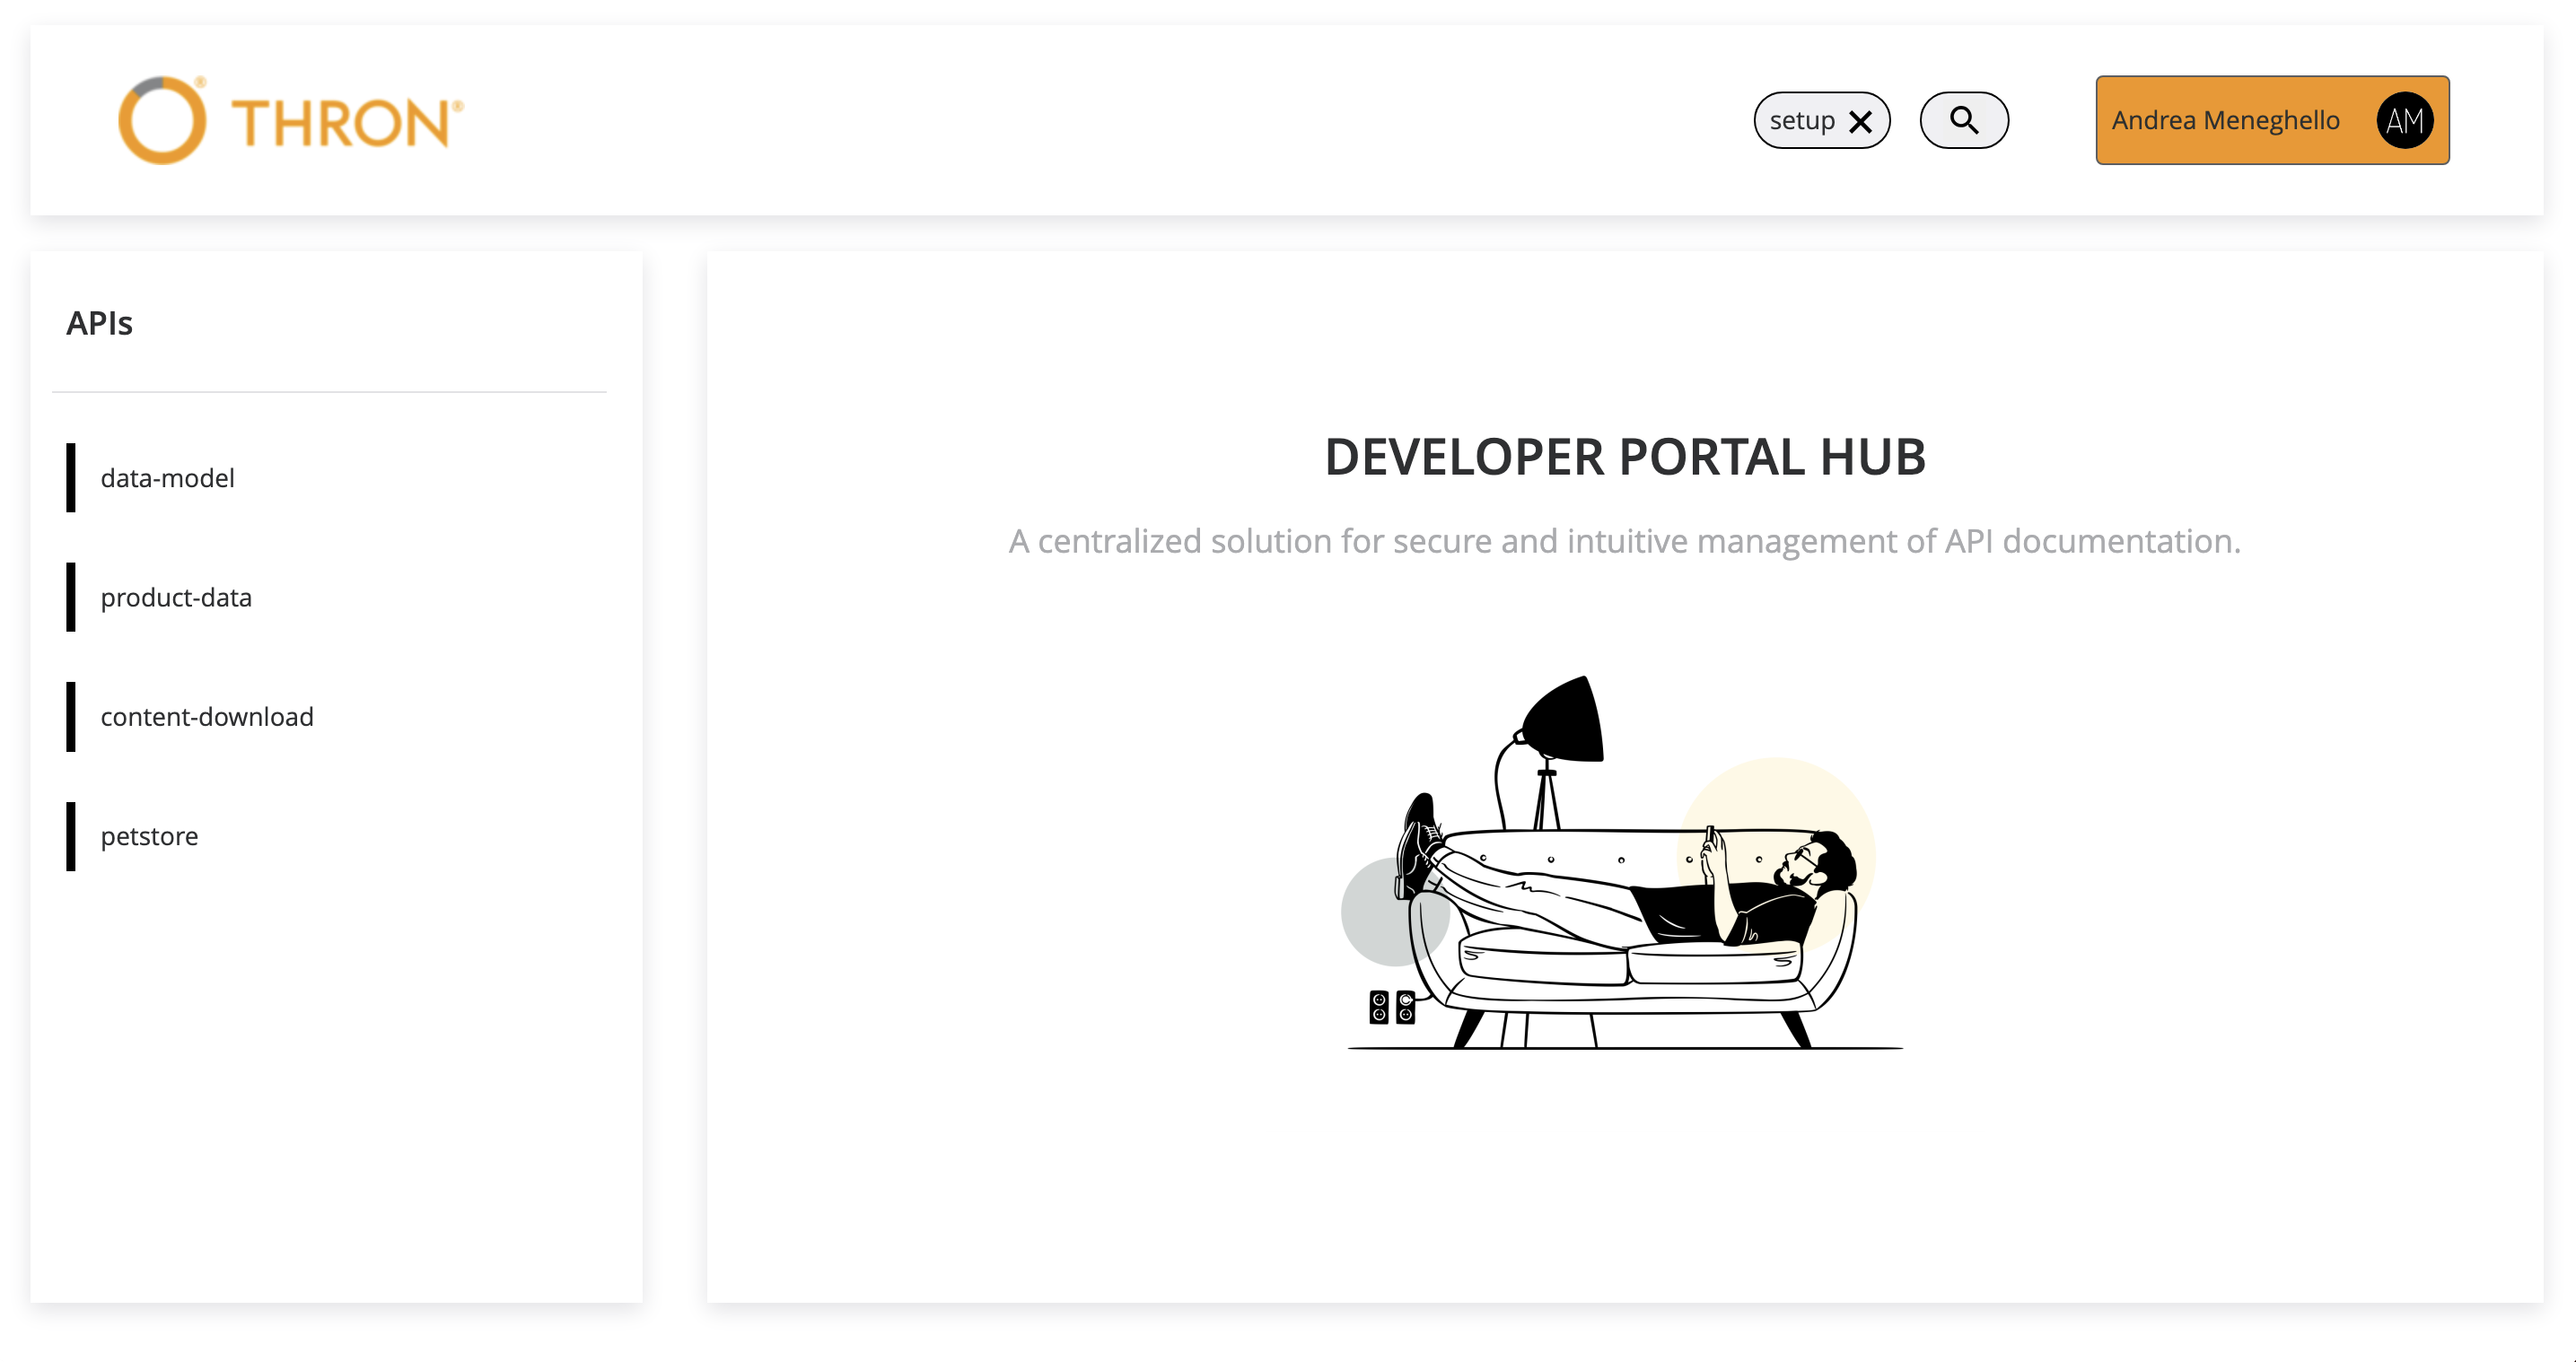
\includegraphics[width=0.6\textwidth, alt={Pagina principale dell'applicazione}]{images/frontend/HomeView.jpg}
  \caption{LoginView}\label{fig:home-view}
\end{figure}

\paragraph{NotFoundView}\label{par:not-found-view}
NotFoundView testo

\begin{figure}[ht]
  \centering
  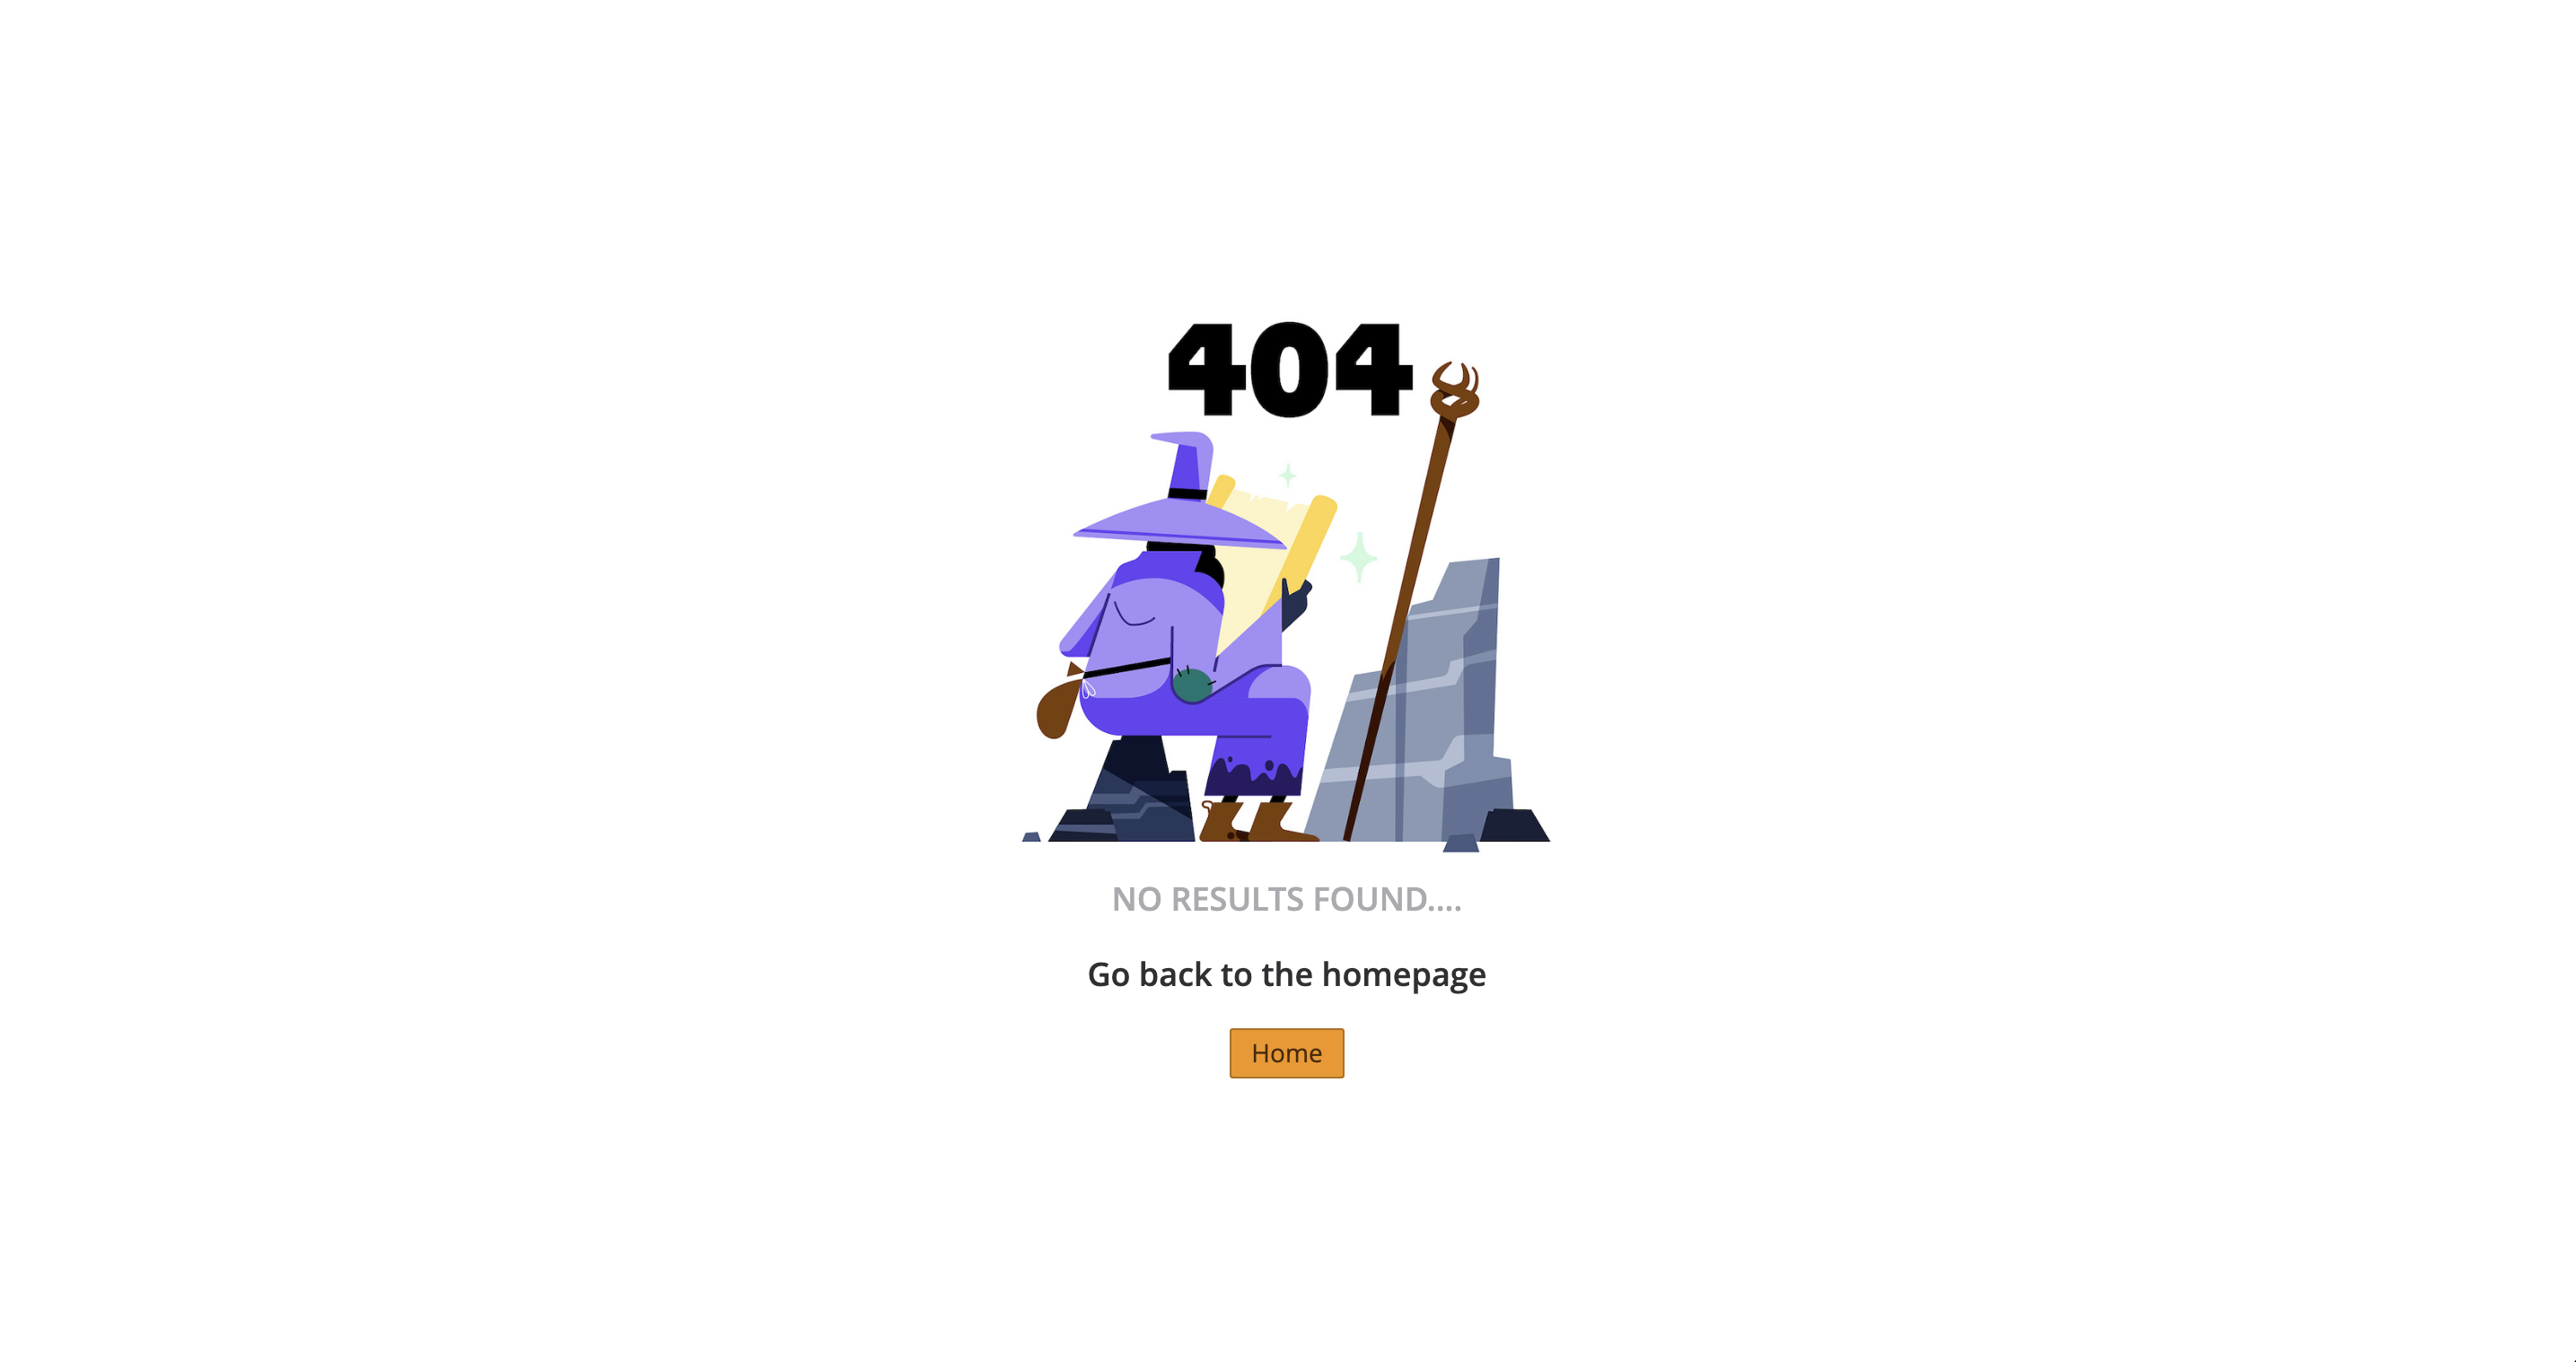
\includegraphics[width=0.6\textwidth, alt={Pagina di errore 404}]{images/frontend/NotFoundView.jpg}
  \caption{NotFoundView}\label{fig:not-found-view}
\end{figure}

\subsubsection{Components}\label{subsubsec:components}

% Home
\paragraph{HeaderNav}\label{par:header-nav}

HeaderNav testo

\paragraph{MainContent}\label{par:main-content}
%swagger
Swagger testo

\paragraph{SideBar}\label{par:side-bar}

Sidebar testo

\paragraph{StartPage}\label{par:start-page}

Start page testo

\paragraph{SwaggerLoader}\label{par:swagger-loader}

Swagger loader testo
\begin{figure}[ht]
  \centering
  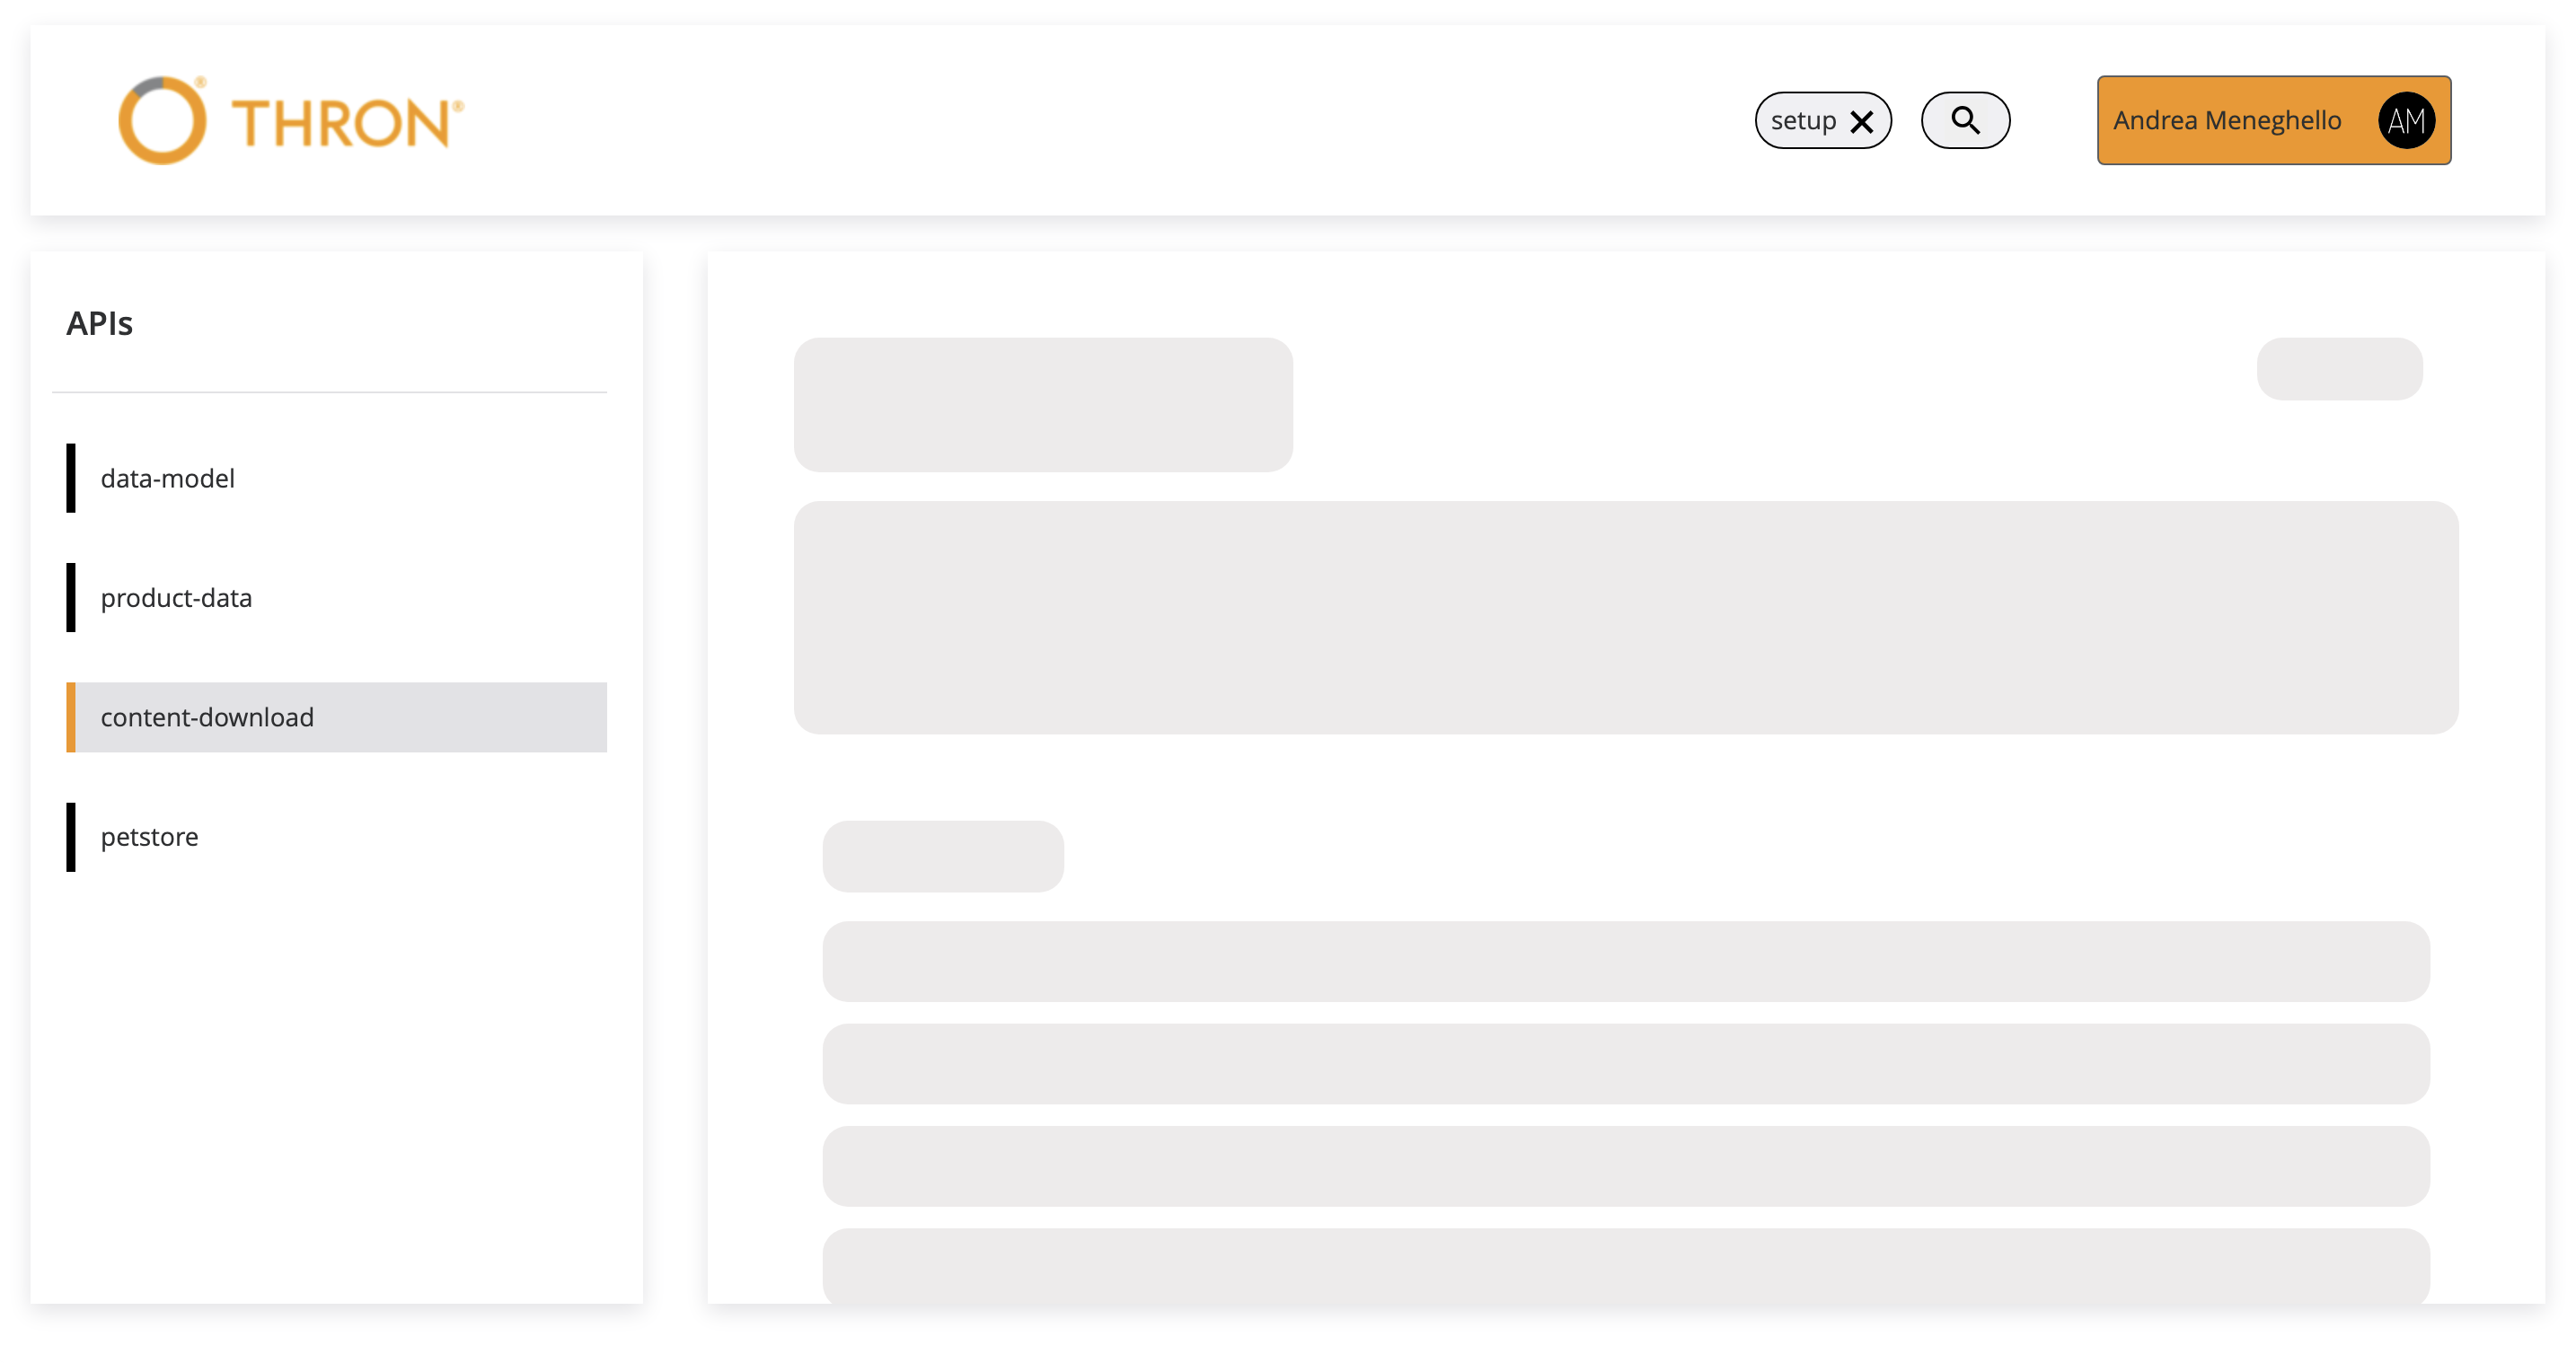
\includegraphics[width=0.6\textwidth, alt={Skeleton loader di caricamento per contenuto principale}]{images/frontend/SwaggerLoader.jpg}
  \caption{SwaggerLoader}\label{fig:swagger-loader}
\end{figure}

\paragraph{DownloadButton}\label{par:download-button}

download button testo

\paragraph{LogoutButtom}\label{par:logout-button}

logout button testo

% Login
\paragraph{LoginButton}\label{par:login-button}

login button testo

% Components
\paragraph{SearchButton}\label{par:search-button}

SearchButton testo

\paragraph{SearchBar}\label{par:search-bar}

Search bar testo

\begin{figure}[ht]
  \centering
  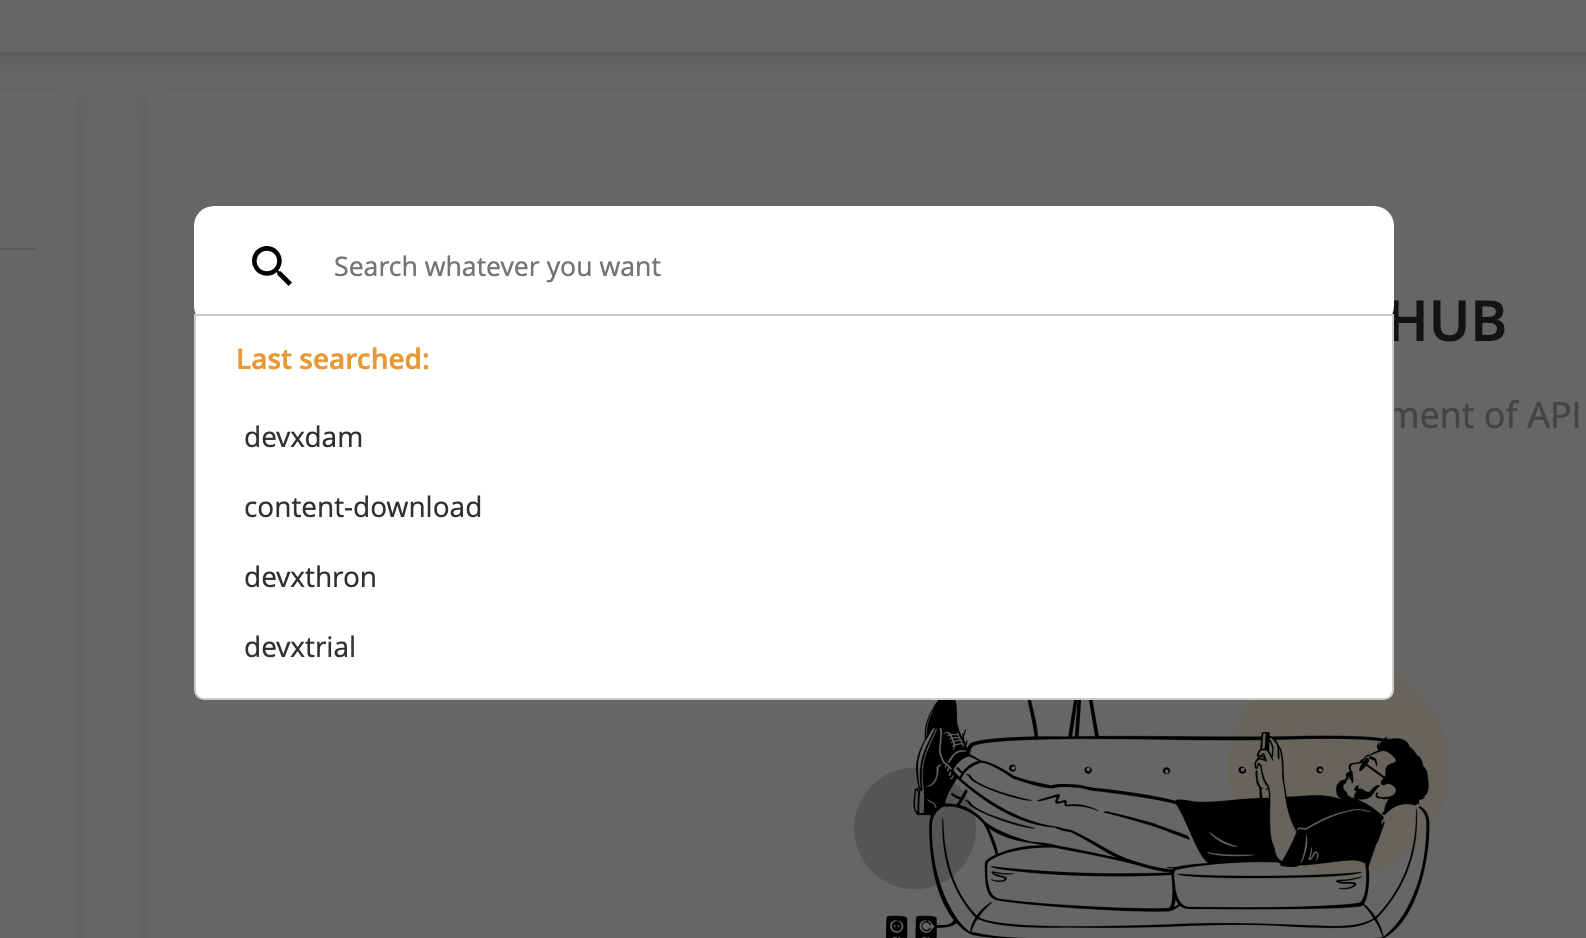
\includegraphics[width=0.6\textwidth, alt={Barra di ricerca globale dell'applicazione}]{images/frontend/SearchBar.jpg}
  \caption{SearchBar}\label{fig:search-bar}
\end{figure}

\paragraph{Autocomplete}\label{par:autocomplete}

Autocomplete testo

\begin{figure}[ht]
  \centering
  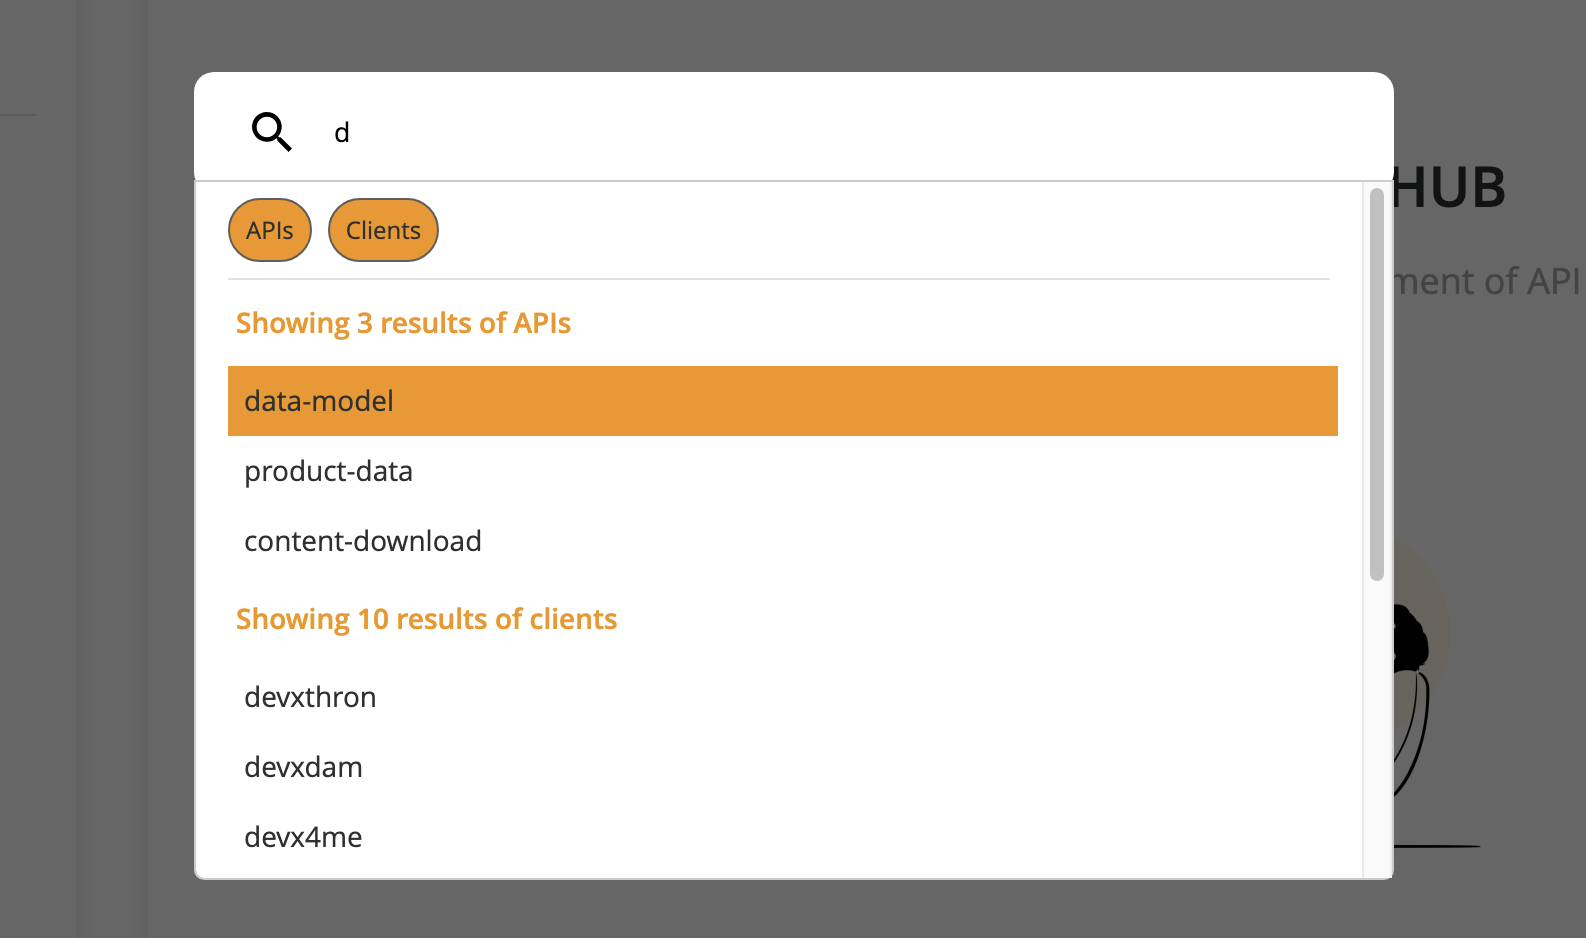
\includegraphics[width=0.6\textwidth, alt={Componente che si occupa della lista dinamica di risultati}]{images/frontend/SearchBar2.jpg}
  \caption{Autocomplete}\label{fig:autocomplete}
\end{figure}

\paragraph{Chip}\label{par:chip}

chip testo da scrivere

\begin{figure}[ht]
  \centering
  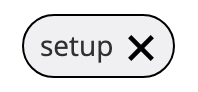
\includegraphics[width=0.3\textwidth, alt={Chip contenente il client id corrente}]{images/frontend/Chip.jpg}
  \caption{Chip}\label{fig:chip}
\end{figure}

\paragraph{Filter}\label{par:filter}

filter testo

\paragraph{OptionList}\label{par:option-list}

option list testo

\paragraph{OptionListItem}\label{par:option-list-item}

OptionListItem testo

\paragraph{SnackBar}\label{par:snack-bar}

snack bar testo da scrivere

\begin{figure}[ht]
  \centering
  
\includegraphics[width=0.3\textwidth, alt={Snackbar di errore}]{images/frontend/SnackBar1.jpg}
  \caption{SnackBar}\label{fig:snack-bar}
\end{figure}

\paragraph{Loader}\label{par:loader}

Loader testo da scrivere

\begin{figure}[ht]
  \centering
  
\includegraphics[width=0.6\textwidth, alt={Skeleton loader di caricamento principale dell'applicazione}]{images/frontend/Loader.jpg}
  \caption{Loader}\label{fig:loader}
\end{figure}



% \subsubsection{Components}\label{:components}
% \subsubsection{Views}\label{subsubsec:views}

\subsection{Codifica back-end}\label{subsec:codifica-back-end}



